\documentclass{article}

\PassOptionsToPackage{svgnames}{xcolor}

\usepackage{tikz}
\usetikzlibrary{
  braids,
  calc,
  intersections,
  spath3
}

% Didn't end up using this, but saving it as it might be useful elsewhere
\tikzset{
  insert node into path/.code n args={3}{%
    \node[spath/save global=node path] at (spath cs:{#1} #2) {#3};
    \tikzset{spath/split globally at intersections with={#1}{node path}}
  }
}


\begin{document}

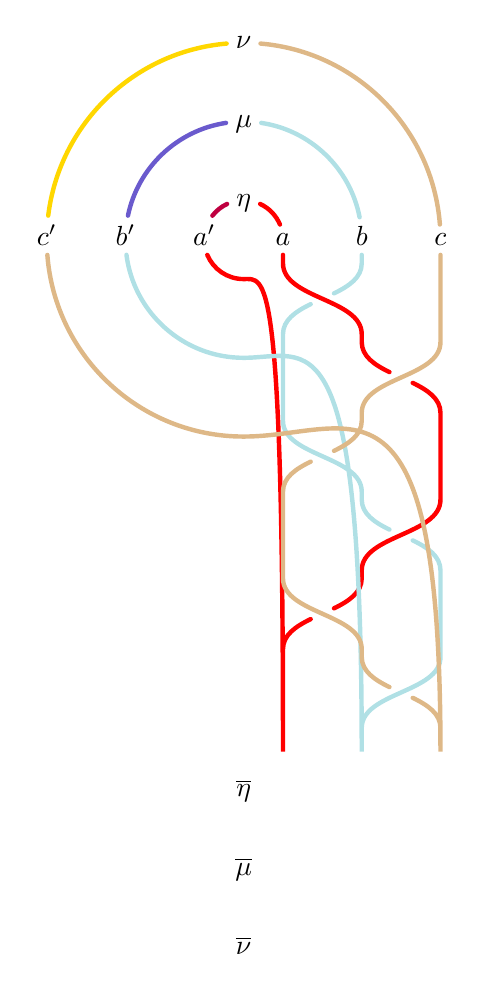
\begin{tikzpicture}[
  every node/.style={anchor=mid},
  every path/.style={line cap=round}
]
  
\pic[
  braid/.cd,
  gap=.1,
  strand 1/.style={draw=none,spath/save global=strand 1},
  strand 2/.style={draw=none,spath/save global=strand 2},
  strand 3/.style={draw=none,spath/save global=strand 3},
] (braid) {braid={s_1 s_2^{-1} s_1 s_2^{-1} s_1 s_2^{-1}}};

\coordinate (a) at (braid-1-s);
\coordinate (b) at (braid-2-s);
\coordinate (c) at (braid-3-s);

\path (braid-1-s) ++(-1,0) coordinate (a');
\path (braid-2-s) ++(-3,0) coordinate (b');
\path (braid-3-s) ++(-5,0) coordinate (c');

\coordinate (toppt) at ($(a.base)!.5!(a'.base)$);
\path (braid-1-e) ++(-.5,0) coordinate (botpt);

\node[spath/save global=a] at (a) {\(a\)};
\node[spath/save global=b] at (b) {\(b\)};
\node[spath/save global=c] at (c) {\(c\)};
\node[spath/save global=a'] at (a') {\(a'\)};
\node[spath/save global=b'] at (b') {\(b'\)};
\node[spath/save global=c'] at (c') {\(c'\)};

\path ($(toppt)!1!90:(a.base)$) node[spath/save global=eta] {\(\eta\)};
\path ($(toppt)!1!90:(b.base)$) node[spath/save global=mu] {\(\mu\)};
\path ($(toppt)!1!90:(c.base)$) node[spath/save global=nu] {\(\nu\)};

\path ($(botpt)!1!-90:(braid-1-e)$) node[spath/save global=etabar] {\(\overline{\eta}\)};
\path ($(botpt)!1!-90:(braid-2-e)$) node[spath/save global=mubar] {\(\overline{\mu}\)};
\path ($(botpt)!1!-90:(braid-3-e)$) node[spath/save global=nubar] {\(\overline{\nu}\)};

\path[spath/save=complete strand 1] ([xshift=-1cm]braid-1-s) coordinate (st) arc[radius=.5, start angle=180, end angle=0] [spath/use={strand 1,weld}] arc[radius=.5cm, start angle=0, end angle=-180] -- (st);
\path[spath/save=complete strand 2] ([xshift=-3cm]braid-2-s) coordinate (st) arc[radius=1.5, start angle=180, end angle=0] [spath/use={strand 2,weld}] arc[radius=1.5cm, start angle=0, end angle=-180] -- (st);
\path[spath/save=complete strand 3] ([xshift=-5cm]braid-3-s) coordinate (st) arc[radius=2.5, start angle=180, end angle=0] [spath/use={strand 3,weld}] arc[radius=2.5cm, start angle=0, end angle=-180] -- (st);

\tikzset{
  spath/remove empty components={complete strand 1},
  spath/split at intersections with={complete strand 1}{a},
  spath/split at intersections with={complete strand 1}{etabar},
  spath/split at intersections with={complete strand 1}{a'},
  spath/split at intersections with={complete strand 1}{eta},
  spath/get components of={complete strand 1}{\innerCpts},
}

\draw[
  ultra thick,
  purple,
  spath/use=\getComponentOf\innerCpts{2},
  spath/use=\getComponentOf\innerCpts{10}
];
\draw[
  ultra thick,
  red,
  spath/use=\getComponentOf\innerCpts{4},
  spath/use=\getComponentOf\innerCpts{6},
  spath/use=\getComponentOf\innerCpts{7},
  spath/use=\getComponentOf\innerCpts{8},
];

\tikzset{
  spath/remove empty components={complete strand 2},
  spath/split at intersections with={complete strand 2}{b},
  spath/split at intersections with={complete strand 2}{mubar},
  spath/split at intersections with={complete strand 2}{b'},
  spath/split at intersections with={complete strand 2}{mu},
  spath/get components of={complete strand 2}{\innerCpts},
}

\draw[
  ultra thick,
  SlateBlue,
  spath/use=\getComponentOf\innerCpts{2},
  spath/use=\getComponentOf\innerCpts{10}
];
\draw[
  ultra thick,
  PowderBlue,
  spath/use=\getComponentOf\innerCpts{4},
  spath/use=\getComponentOf\innerCpts{6},
  spath/use=\getComponentOf\innerCpts{7},
  spath/use=\getComponentOf\innerCpts{8},
];

\tikzset{
  spath/remove empty components={complete strand 3},
  spath/split at intersections with={complete strand 3}{c},
  spath/split at intersections with={complete strand 3}{nubar},
  spath/split at intersections with={complete strand 3}{c'},
  spath/split at intersections with={complete strand 3}{nu},
  spath/get components of={complete strand 3}{\innerCpts},
}

\draw[
  ultra thick,
  Gold,
  spath/use=\getComponentOf\innerCpts{2},
  spath/use=\getComponentOf\innerCpts{10}
];
\draw[
  ultra thick,
  BurlyWood,
  spath/use=\getComponentOf\innerCpts{4},
  spath/use=\getComponentOf\innerCpts{6},
  spath/use=\getComponentOf\innerCpts{7},
  spath/use=\getComponentOf\innerCpts{8},
];

\end{tikzpicture}
\end{document}

\path[spath/save=complete strand 1] (spath cs:{strand 1} 0) ++(-1,0) coordinate (a) arc[radius=.5cm, start angle=180, end angle=0] [spath/use={strand 1,weld}] arc[radius=.5cm, start angle=0, end angle=-180] -- (a);

\tikzset{
  spath/remove empty components={complete strand 1},
  insert node into path={complete strand 1}{0}{\(a'\)},
  insert node into path={complete strand 1}{.1}{\(\eta\)},
  insert node into path={complete strand 1}{.26}{\(a\)},
  insert node into path={complete strand 1}{.865}{\(\bar{\eta}\)},
  spath/get components of={complete strand 1}{\innerCpts}
}

\draw[
  ultra thick,
  purple,
  spath/use=\getComponentOf\innerCpts{2},
  spath/use=\getComponentOf\innerCpts{10}
];
\draw[
  ultra thick,
  red,
  spath/use=\getComponentOf\innerCpts{4},
  spath/use=\getComponentOf\innerCpts{6},
  spath/use=\getComponentOf\innerCpts{7},
  spath/use=\getComponentOf\innerCpts{8},
];

\draw[ultra thick, orange] (spath cs:{strand 2} 0) ++(-3,0) coordinate (a) arc[radius=1.5cm, start angle=180, end angle=0] [spath/use={strand 2,weld}] arc[radius=1.5cm, start angle=0, end angle=-180] -- (a);

\draw[ultra thick, blue] (spath cs:{strand 3} 0) ++(-5,0) coordinate (a) arc[radius=2.5cm, start angle=180, end angle=0] [spath/use={strand 3,weld}] arc[radius=2.5cm, start angle=0, end angle=-180] -- (a);


\end{tikzpicture}

\end{document}
